\documentclass{/home/janmebows/Documents/LatexTemplates/myassignment}


\title{Modelling with ODEs Assignment 2}
\begin{document}

\maketitle
\begin{enumerate}
    \item 
    \begin{enumerate}
        \item $\dot x = r + x - \log (1+x)$
        % Bifurcation Value
        Bifurcation when $f(x:r) = r+x-\log(1+x) = 0$ and $f'(x:r) = 0$ the solutions $(x,r)$ are the bifurcation point value pair.
        \begin{align*}
            f(x:r) = r+ x - \log(1+x) &= 0\\
            r = \log(1+x) - x\\
            f'(x:r) = 1 - \frac1{1+x} &=0\\
            \implies x = 0\\
            f(0:r) = 0
        \end{align*}
        So the bifurcation value is $\bar{r} = 0$ at $(\bar{x},\bar{r}) = (0,0)$
       
        %  Type
        For $r<0$ there are 2 fixed points for $x$. The fixed points with $x >0$ will produce 
        \[\dot x > 0\]
        Which implies they will be unstable. The values where $x < 0$ will give
        \[\dot x < 0\]
        And thus they are stable.
        For $r =0$ there is only 1 fixed point (the bifurcation), and for $r >0$ there are no fixed points.
        This is all shown in figure~\ref{fig:q1a}. Hence this is a saddle node bifurcation.


        %   Bifurcation Diagram
         \begin{figure}[H]
             \centering
             \label{fig:q1a}
             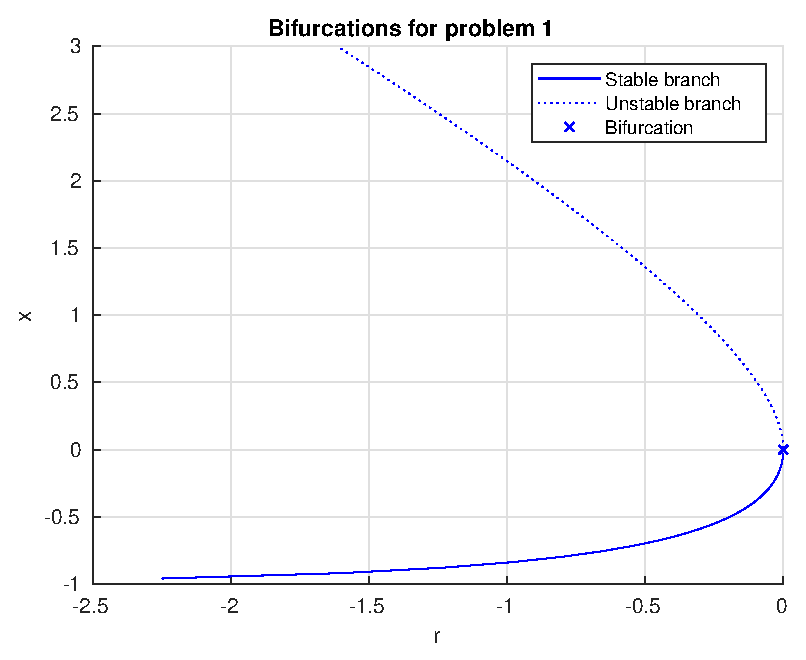
\includegraphics{ODEsA2Q1a.eps}
             \caption{Bifurcation diagram for $\dot x = r + x - \log (1+x)$}
         \end{figure}

         As shown in figure~\ref{fig:q1a}, the stable solution disappears after the bifurcation, and the branch of fixed points is unstable.


        \item $\dot x = x-rx (1-x)$
        %Bifurcation Value
        \begin{align*}
            f(x:r) = x - rx(1-x) &=0\\
            x(1-r(1-x)) = 0\\
            x =0 \ &or \ r-rx-1 =0\\
            x = 0 \ &or \ x = 1-\frac{1}{r}\\
            f'(x:r) = 1 - r - 2rx &=0\\
            1 -r = 0 \ &or \ 1 - r - 2r(1 - \frac1r) = 0\\
            r = 1 \ &or \ 1-3r+ 2 = 0\\
            \implies r = 1 
        \end{align*}
        
        %Type
        Noting $f'(x:r) = 1-r-2rx$, we get $x=0$, $r>1$ is stable, $x=0$, $r <1$ is unstable. For $x = 1-1/r$, $r > 0$ it is unstable, and the same $x$ for $r <0$ is stable. So this suggests that this is a transcritical bifurcation.
        %Bifurcation Diagram         
        \begin{figure}[H]
             \centering
             \label{fig:q1b}
             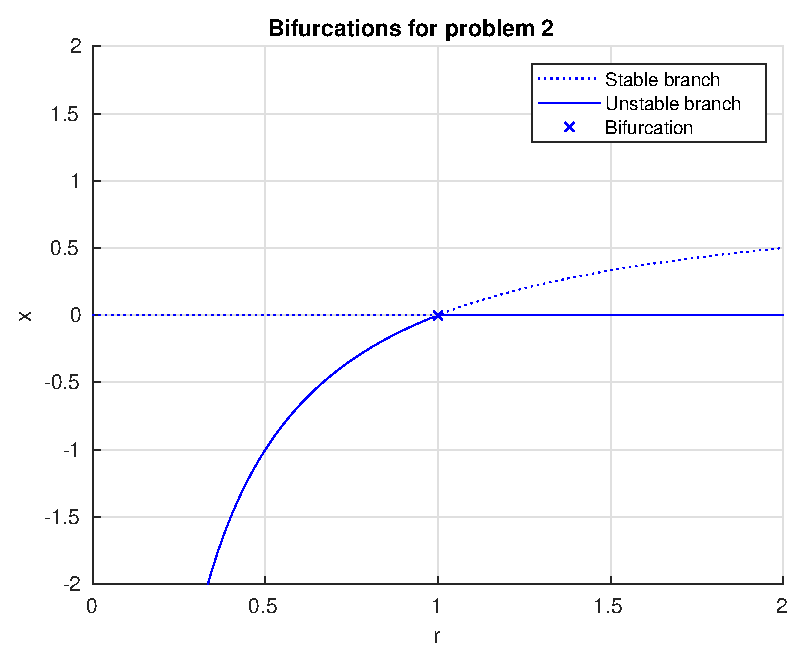
\includegraphics{ODEsA2Q1b.eps}
             \caption{Bifurcation diagram for $\dot x = x-rx (1-x)$}
         \end{figure}

        Figure~\ref{fig:q1b} is the bifurcation diagram for this problem. This is a form of a transcritical bifurcation, since on both sides of the bifurcation there is one stable and an unstable fixed point.


        \item $\dot x = rx - 4x^3$
        %Bifurcation Value
        \begin{align*}
            \dot x = 0\\
            x(r - 4x^2) = 0\\
            x = 0 \quad x = \pm\frac12\sqrt r
        \end{align*}
        %Type
        
        %Bifurcation Diagram
        \begin{figure}[H]
             \centering
             \label{fig:q1c}
             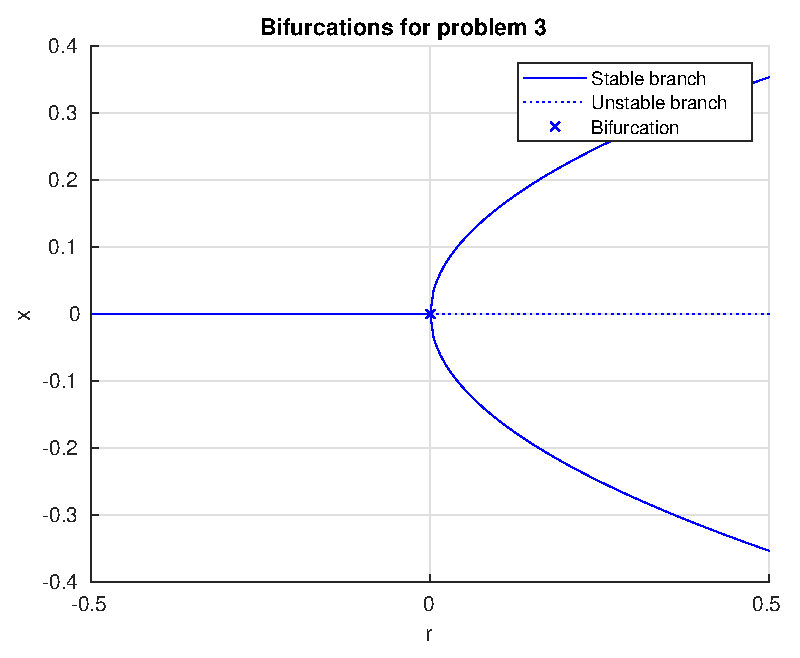
\includegraphics{ODEsA2Q1c.eps}
             \caption{Bifurcation diagram for $\dot x = rx - 4x^3$}
         \end{figure}
         Figure~\ref{fig:q1c} is the bifurcation diagram for this. Note that from observation the problem was very similar to the canonical form for the supercritical pitchfork bifurcation. Clearly this is a supercritical pitchfork bifurcation as after $r$ is increased past the bifurcation point, the one stable branch splits into 2 stable branches and an unstable branch.

    \end{enumerate}

    %%%Question 2
    \item 
    \begin{enumerate}
        \item Since $r=0.4$, $x(0)=0$ the ODE becomes
        \[\frac{dx}{d\tau} = s - 0.4 x + \frac{x^2}{1+x^2}\]
    \begin{enumerate}
        \item %what happens to x(\tau) and why
        There is a bifurcation point which is crossed when $s$ is increased towards $0.2$.
        Before this bifurcation point, the system will remain with no gene product, i.e. $x\tau =0$. This is because $x=0$ is a stable fixed point. After $s$ is increased to the bifurcation value, the fixed point becomes semistable 
        Since $\frac{dx}{d\tau}\Bigm|_{x=0} = s$. Expect a positive slope about $x=0$. 
        Note $x < 0$ cannot occur since when $x\to 0$, $ s > x$ and hence $\frac{dx}{d\tau} > 0$. So $x$ will always be greater than zero 
        When $s = 0.2$ 

        The bifurcation point, where the stability is lost:
        \begin{align*}
            0&=-0.4 + \frac{2x(1+x^2) -2x^3}{(1+x^2)^2} \\
            &=-0.4 + \frac{2x}{(1+x^2)^2} \\
            2x &= 0.4(1+2x^2 +x^4)
        \end{align*}
        Which is not analytic.
        Solving for the first smallest positive solution numerically in \verb|Matlab| yields $\bar{x} \approx 0.2198$ And hence $\bar{s} \approx 0.0418$. This is a semi-stable fixed point.
        Once $s>\bar{s}$, $x$ is allowed to jump up to a much larger value I.e. $x \gg \bar{x}$.

        Once $s$ reaches $0.2$, $x$ will eventually reach its maximum at $2.6981$ (obtained from \verb|Matlab|). This is a stable fixed point (identifiable from figure~\ref{fig:q2b1}). 


        \begin{figure}[H]
             \centering 
             \label{fig:q2b1}
             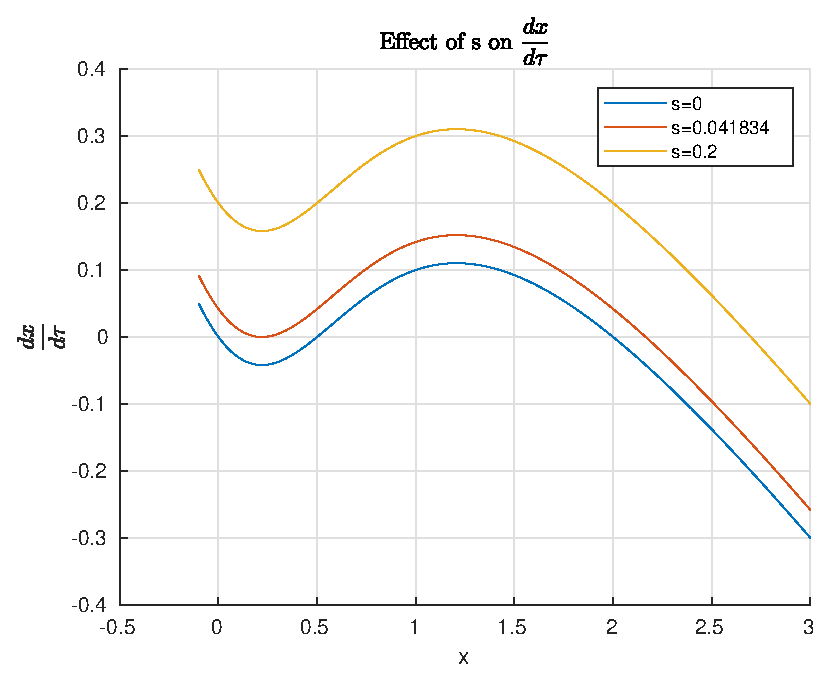
\includegraphics{ODEsA2Q2a.eps}
             \caption{plot of $\frac{dx}{d\tau}$ against $x$, for $s=0$ $\bar{s}$, and $s=0.2$}
         \end{figure}
        \item %what happens if we now decrease s back towards zero
        If $s$ is now decreased back to $0$, $x$ will shift left due to the negative derivative. The derivative becomes zero for $s=0$, and $\tilde{x} = 2$. This is a stable fixed point since the slope of $\frac{dx}{dt}$ is negative around this point.

        The fact that increasing $s$ and then decreasing it gives different steady states suggests there is hysteresis.
        %grab a bifurcation plot and show stability (hysteresis?)
    \end{enumerate}
        \item Now we are varying both $s$ and $r$ in 
        \[\frac{dx}{d\tau} = s - r x + \frac{x^2}{1+x^2}\]
        Noting that $r>0$ and $s \geq 0$.
    \begin{enumerate}
        \item %Calculate Bifurcation curves
        \begin{align*}
            f(x:s,r) = s - rx + \frac{x^2}{1+x^2} =0\\
            f'(x:s,r) = -r +    \frac{2x}{(x^2+1)^2} =0\\
            \implies r = \frac{2x}{(x^2+1)^2}\\
            \implies s - \frac{2x^2}{(x^2+1)^2} + \frac{x^2}{1+x^2} =0\\
            \implies s =\frac{2x^2}{(x^2+1)^2} - \frac{x^2}{1+x^2} \\
            \implies s = \frac{x^2(1-x^2)}{(x^2+1)^2}
        \end{align*}
        So the bifurcation curves are
        \[r = \frac{2x}{(x^2+1)^2}, \quad s = \frac{x^2(1-x^2)}{(x^2+1)^2} \]
        \item %Plot bifurcation curves $r(x)$, $s(x)$.
        \begin{figure}[H]
             \centering
             \label{fig:q2b2}
             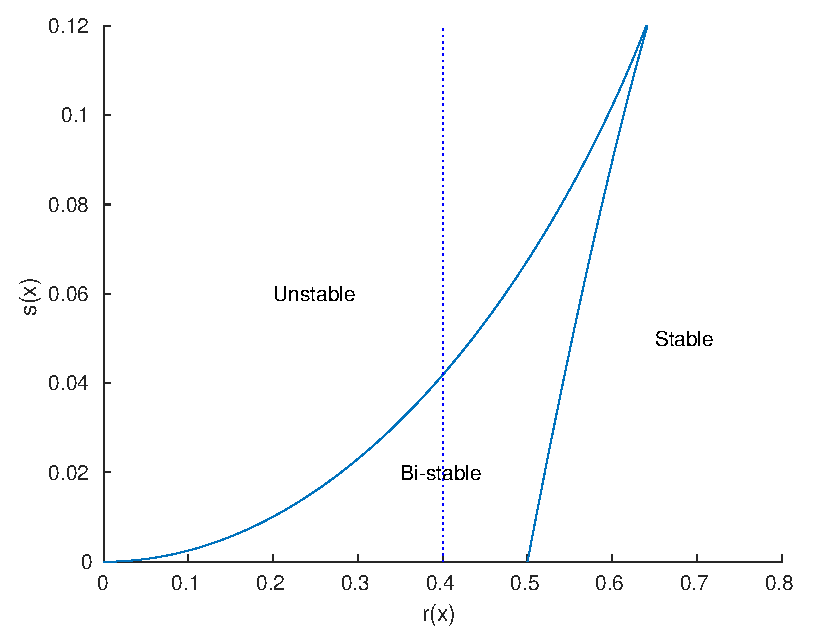
\includegraphics{ODEsA2Q2b.eps}
             \caption{Bifurcation curves, in the $r(x)$, $s(x)$ plane. Dotted line at $r=0.4$}
         \end{figure}
        Figure~\ref{fig:q2b2} plots the bifurcations in the $(r,s)$ plane. The dotted line for $r=0.4$ shows the nature of the previous problem. Where fixing $r=0.4$ and increasing $s$ to $0.2$ made the problem move from the bi-stable region to the unstable region, and then decreasing it led it back into the bi-stable region.

        
        \item %Number of steady states an stability. What happens along the bifurcation curves
        The example in question 2a had $s = 0.2$, $r=0.4$. It is clear that this lies in the unstable region. This can be seen visualy from the plot~\ref{fig:q2b2}.

        The curve for $r(x)$, $s(x)$ is the bifurcation for the system. Along the curve there exists 2 steady states. On the region contained within the curve (the bistable region), there are 3 steady states, and outside of the curve there is only 1 steady state. These are demonstrated in figure~\ref{fig:q2b1}, the $s=0$ plot sits within the bistable region, the $s\approx 0.041834$ sits on the bifurcation curve, and only has one steady state, and the $s=0.2$ is in the unstable region (outside of the steady state curve) and there is only 1 solution.

    \end{enumerate}
    \end{enumerate}
\end{enumerate}

\clearpage

\section*{Matlab Code}
\lstinputlisting{ODEsA2.m}

\clearpage
\includepdf[pages=1-]{A2_2019.pdf}

\end{document}
